
\chapter{Particle Finite Element Methods for the shallow water equations}
\label{lagrangian_sw}




In chapter \ref{eulerian_sw} the SW equations have been analyzed considering the coupled convective and oscillatory mechanisms in an Eulerian framework. However, in some regions of the domain, the solution of the equations can be convection dominated. Specifically, whenever there is a movement of the shoreline --like run-up or flooding--, the problem is convection dominated.
This mechanism suggests the use of Lagrangian strategies, which have been successfully applied to convection diffusion and Navier-Stokes problems.

In this appendix, the developments of the Particle Finite Element Method (PFEM) are applied to the SW equations. The basis of the PFEM family of methods consists on a splitting operator, solving two stage fashion the convective operator and the rest of the equations. In the case of the SW equations, there is a stage for convection and other stage for wave mechanism.
The main advantage of the PFEM lies in using the variational principle of FEM. Hence, the formulations presented in chapter \ref{eulerian_sw} are applicable with small modifications. The novelty of the PFEM consists on solving the convection with a particle method.

In the family of PFEM there are two main groups, the moving mesh and the fixed mesh. The mesh moving algorithm was firstly presented to the scientific community \cite{idelsohn2003,idelsohn2004} and has been widely applied to a high number of situations \cite{larese2008,Salazar2012,onate2008}. In this method, the particles traditionally coincide with the nodes. After the convection stage --and eventually, remeshing--, the mesh inherits the displacements of the convection. Those displacements are part of the material derivative involved in the variational principle of the equations.

Lately, a second generation of the PFEM was presented \cite{idelsohn2012}. It uses a fixed mesh and is known as PFEM-2. The main idea consists on decoupling the particles from the nodes, leading to a duality of spaces: the FEM discretization and the particles discretization. Its main drawback is the introduction of projections between the two spaces but the cost of the projection is expected to be compensated by the use of a fixed mesh strategy without remeshing \cite{idelsohn2015,puigferrat2021}.



\section{Introduction}

The Lagrangian formulation starts by the definition of the material derivative. Let $\varphi$ be a scalar or vector property, the material derivative is obtained by applying the chain rule:
\begin{subequations} \label{mat_derivative}
\begin{align}
\frac{D}{Dt}\varphi(\mathbf{x},t) &= \pder{\varphi}{t} + u\cdot\nabla\varphi \label{mat_derivative:deriv} \\
\pder{\mathbf{x}}{t} &= \mathbf{u} \label{mat_derivative:conv}
\end{align}
\end{subequations}
The Lagrangian procedure consist on solving separately the equations (\ref{mat_derivative:deriv}) and (\ref{mat_derivative:conv}). To apply this staggered procedure, a generic conservation balance is considered,
\begin{equation} \label{conserv_balance}
\pder{\varphi}{t} + \nabla \mathbf{F} = 0
\end{equation}
where $\mathbf{F}$ is the fluxes vector in an infinitesimal volume of control. The balance equation is split into the convective and non convective fluxes, $\mathcal{L}_1$ and $\mathcal{L}_2$ respectively.
\begin{equation} \label{spatial_balance_linearized}
    \pder{\varphi}{t} + \mathcal{L}_1 \varphi + \mathcal{L}_2 \varphi = 0
\end{equation}
After introducing equation (\ref{mat_derivative}) into (\ref{spatial_balance_linearized}), the following expression is obtained,
\begin{equation} \label{mat_balance_liearized}
    \frac{D\varphi}{Dt} + \mathcal{L}_2 \varphi = 0
\end{equation}

Finally, the numerical strategy for solving a balance equation (\ref{conserv_balance}) in a Lagrangian framework consists on applying a splitting, generally, the first order Godunov splitting \cite{leveque2002} or the second order Strang splitting \cite{macnamara2016}.
The order of accuracy of the splitting operator is related to the sequence and the mode how equations (\ref{mat_derivative:conv}) and (\ref{mat_balance_liearized}) are temporally integrated.





\section{Mesh moving methods}


The PFEM method has been widely applied to solve the incompressible Navier-Stokes equations, especially with free surface problems \cite{larese2008}, multi-fluids \cite{mier2010} and fluid-structure interaction \cite{onate2008}.
The moving mesh allows to fit the sub-domains with the discretization and the boundaries are tracked in a natural way.
When the PFEM is applied to the SW equations, the mesh moving will be solving the water domain in the horizontal plane. That is, the moving shoreline in the SW equations is playing the role of the free surface in the NS equations.

Once the discretization describes and follows the fluid motion --$\eta$ and $\mathbf{u}$--, there appears the need to introduce another discretization to define the fixed topography and its variations --$z$--, since it does not move with the fluid. The duality of discretizations introduce the need of a mapping between the two meshes. The topography data need to be mapped to the computational mesh for solving the equations. And the primal variables need to be mapped to the topographical mesh for visualization purpose. See figure \ref{pfem_dual_mesh}, where the fluid domain $\Omega_w$ si inside the computational domain $\Omega$. The topographic domain $\Omega_T$ coincides with the computational domain $\Omega$.
This approach presents some analogies with embedded formulations, except on the fact that the discontinuity is on the fluid --computational domain-- instead of the topography --geometric domain--.


\begin{figure} [ht]
    \centering
    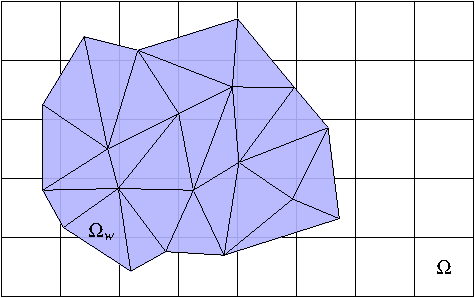
\includegraphics[width=.6\textwidth]{img/lagrangian/dual_pfem_mesh.pdf}
    \caption{Spatial discretization for the mesh moving PFEM algorithm.}
    \label{pfem_dual_mesh}
\end{figure}

Going back to the definition of the SW flow, the set of particles moving in the Lagrangian frame, convect the intrinsic properties (density, water depth, velocity, flow rate, etc.). The equations follow an \emph{updated lagrangian} formulation, that is, the variables are assumed to be known at time $t$ but unknown for the time $t+\Delta t$. Given that the variational principle is used to solve the equations in the continuum media, those is identified with the fluid domain, excluding the dry part. Once the convection is solved and the shoreline is updated, the system of equations is solved again.

Some modifications to this procedure may be considered. For example, an excessive deformation of the elements, without inverting them, may require a remeshing step. In that case, the identification of the shoreline coincides with the previous time step, but the interior domain will be refined. With a proper mesh quality control, the remeshing step can be applied only to those steps which really need it.

Additionally, an iterative scheme can be introduced, since the solution of the nwe system of equations at time step $t + \Delta t$ modifies the integration of the convective term. Usually this outer iteration loop is skipped by an explicit approximation of the convective term. The full path of the solution procedure is resumed in figure \ref{sw_pfem_algorithm}.

\begin{figure} [ht]
    \centering
    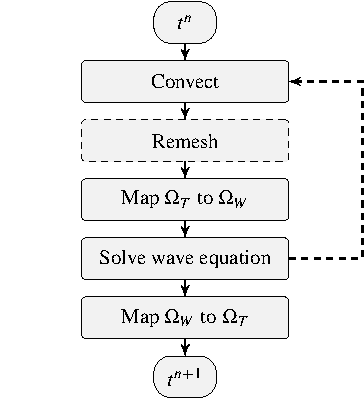
\includegraphics[width=.6\textwidth]{img/lagrangian/sw_pfem_algorithm.pdf}
    \caption{PFEM algorithm for the SW equations.}
    \label{sw_pfem_algorithm}
\end{figure}





\subsection{Governing equations}


Given that the nodes of the SW discretization are particles, the intrinsic properties are in a Lagrangian frame, thus, both mass and momentum balances follow a Lagrangian formulation. This fact reduces the non-linearity of the system of equations to be solved, making them easier to solve. On the other hand, in the Lagrangian framework the convection can be evaluated in terms of the primitive variables. We will take advantage of this characteristic to solve the primitive SW, which are more linear than the conservative ones.
The accuracy of the solutions obtained with the proposed method will be compared against the methods presented in the previous chapter.

Let the conservative vector of unknowns $\bm\phi$ be expressed in terms of the primitive set of variables $\bm\psi$. we recover the SW equations in terms of the primitive variables:
\begin{subequations}
\begin{align}
    \pder{\mathbf{u}}{t} &= \mathbf{u} \cdot \nabla \mathbf{u} + g \nabla(h-z_b) + g\mathbf{S}_f = \mathbf{0} \\
    \pder{h}{t} &= \mathbf{u} \cdot \nabla h + h \nabla \mathbf{u} = 0
\end{align}
\end{subequations}
The introduction of the material derivative definition yields
\begin{subequations} \label{pfem_mat_balance}
\begin{align}
    \frac{D\mathbf{u}}{Dt} &= g \nabla(h-z_b) + g\mathbf{S}_f = \mathbf{0} \\
    \frac{Dh}{Dt} &= h \nabla \mathbf{u} = 0
\end{align}
\end{subequations}

Analogously to the previous sections, if the solution $\psi$ is sufficiently smooth, it will also verify the quasi-linear form
\begin{equation} \label{pfem_mat_balance_lin}
    \frac{D\bm{\psi}}{Dt} + \mathbf{A}_i\pder{\bm{\psi}}{x_i} + \mathbf{S}\bm{\psi} + \mathbf{T} = 0
\end{equation}
Where the matrix $\mathbf{S}$ and the vector $\mathbf{T}$ are the same than those defined in section \ref{equations}. The tangent matrices $\mathbf{A}_i$ have a new expression for this case, according to the change of variables and to the material derivative. The null diagonal corresponds to the non-convective look of the equations.
\begin{equation}
    \mathbf{A}_1 = \left[\begin{array}{ccc}
        0 & 0 & g \\
        0 & 0 & 0 \\
        h & 0 & 0
    \end{array}\right] \quad , \quad
    \mathbf{A}_2 = \left[\begin{array}{ccc}
        0 & 0 & 0 \\
        0 & 0 & g \\
        0 & h & 0
    \end{array}\right]
\end{equation}


The eigenvalues of $\mathbf{A}_i$ for the one-dimensional case are $\lambda = \pm c$, being $c=\sqrt{gh}$ the surface waves speed. These eigenvalues differ from $u+c$ and $u-c$ since we are in a Lagrangian frame, moving at velocity $u$.
For the two-dimensional case, the eigenvalues for each direction are obtained projecting $\mathbf{A}_i$ onto a unit vector and are always $-c$, $0$ and $c$.
The system is still hyperbolic and the positivity of $h$ is required. 




\subsection{Variational principle}


Despite the non-convective look of (\ref{pfem_mat_balance}), they need stabilization because of the incompatibility of the interpolation \cite{codina2008}. The fic-based stabilization method from \cite{onate1998} and from the previous sections will be reused. As stated before, this formulation presents a significative simplification with respect to the conservative equations in an Eulerian frame. The residual of the equations is defined as
\begin{equation}
    \mathbf{r} \defeq \frac{D\bm{\psi}}{Dt} + \mathbf{A}_i\pder{\bm{\psi}}{x_i} + \mathbf{S}\bm{\psi} + \mathbf{T} = 0 \quad i = 1,2
\end{equation}

The number of dimensions is $n_d=2$ and the number of balance equations is $n_b=3$. The FIC-balance using a first order expansion of Taylor series has the following expression:
\begin{equation} \label{fic_expression}
    r_j - \frac{1}{2} l^e \frac{\mathbf{A}_i}{\lambda_{max}} \pder{r_j}{x_i} = 0 \qquad i \in \{1,n_d\} \ , \ j \in \{1,n_b\}
\end{equation}
To introduce stability in the desired direction, the characteristic element length $l^e$ has been projected onto the normalized characteristics of the equation, $\mathbf{A}_i/\lambda_{max}$.
In practice, the term $\frac{1}{2}$ is replaced by an algorithmic constant $\beta$ in order to control the amount of extra diffusion. This parameter will be analyzed latter.


The resulting SW FIC-based stabilization is obtained from (\ref{pfem_mat_balance_lin}) and (\ref{fic_expression}). The variational principle is obtained by multiplying the FIC balance by a test function $\omega_k$ and integrating over the domain $\Omega_w$.
\begin{equation} \label{variational_fic_lagr}
    \int_{\Omega_w} \left(\omega_k \mathbf{r} + \omega_k \beta l^e \frac{\mathbf{A}_i}{\lambda} \pder{\mathbf{r}}{x_i}\right) d\Omega = 0
\end{equation}


The second term of Equation (\ref{variational_fic_lagr}) is integrated by parts. % This was in red. Check the explanation
Note that the geometries are linear and the element length $l^e$ and the linearization matrix $\mathbf{A}_i$ are defined constant inside the element. Hence, the boundary integral which appears after integration by parts should be understood as the boundary of all the elements

\begin{equation} \label{variational_fic_lagr_parts}
\int_{\Omega_w} \omega_k \mathbf{r} d\Omega
- \int_{\Omega_w} \beta l^e\frac{\mathbf{A}_i}{\lambda}\pder{\omega_k}{x_i} \mathbf{r} d\Omega
+ \sum_e \int_{\Gamma_e} \beta l^e\frac{\mathbf{A}_i}{\lambda}\omega_kn_k \mathbf{r} d\Gamma = 0
\end{equation}
In this work we neglect the boundary integrals assuming that the residual $\mathbf{r}$ is null at the boundary of the elements. At this point we introduce the balance Equation (\ref{pfem_mat_balance}) and integrate by parts again. The result is

\begin{multline} \label{variational_balance_fic_lagr}
\int_{\Omega_w} \left(
    \omega_k \pder{\bm{\psi}}{t} + \omega_k \mathbf{A}_i\pder{\bm{\psi}}{x_i}
    + \pder{\omega_k}{x_j} \mathbf{K}_{jk} \pder{\bm{\psi}}{x_i} + \mathbf{S}\bm{\psi} + \mathbf{F}
\right) d\Omega\\ -
\int_{\Omega_w} \frac{\beta l^e}{\lambda} \left(
    \pder{\omega_k}{x_j} \mathbf{A}_j \pder{\bm{\psi}}{t}
    + \pder{\omega_k}{x_j} \mathbf{A}_j\mathbf{A}_i\pder{\bm{\psi}}{x_i}
    + \ppder{\omega_k}{x_j} \mathbf{A}_j\mathbf{K}_{jk} \pder{\bm{\psi}}{x_i} \right. \\
    \left.
    + \pder{\omega_k}{x_j} \mathbf{A}_j(\mathbf{S}\bm{\psi} + \mathbf{F})
\right) d\Omega
=0
\end{multline}
Equation (\ref{variational_balance_fic_lagr}) is the stabilized variational form for the shallow water equations, similar to the expression obtained by SUPG. Note that the parameter $\beta l^e/\lambda$ is analogous to the characteristic time $\tau$ of the classical SUPG or GLS techniques \cite{cotela2016}.



\subsection{Convective operator}


Apart from solving Eq. (\ref{pfem_mat_balance}), Eq. (\ref{mat_derivative:deriv}) needs to be integrated in time. Given that (\ref{mat_derivative:deriv}) does not involve a spatial derivatives, there is no need to use a variational principle and can be evaluated nodally. In other words, the trajectory of the particles is decoupled from the wave.

In order to evaluate the trajectory of the particles, Eq. (\ref{mat_derivative:deriv}) is rewritten in integral form
\begin{subequations}
\begin{align}
    \mathbf{x}(t^{n+1}) &= \mathbf{x}(t^n) + \int_{t^n}^{t^{n+1}} \mathbf{u}(t) dt \\
    \mathbf{u}(t^{n+1}) &= \mathbf{u}(t^n) + \int_{t^n}^{t^{n+1}} \mathbf{a}(t) dt
\end{align}
\end{subequations}


As far as the time variable is evaluated at discrete intervals $t = t^1, \dots t^n$, the continuous value of $t$ is not known. Therefore, a generic finite difference can be used to evaluate the position continuously in time:
\begin{equation}
    \mathbf{x}^{n+1} = \mathbf{x}^n +
        (1-\theta) (\Delta t \mathbf{u}^n + \frac{1}{2} \Delta t^2 \mathbf{a}^n) +
        \theta (\Delta t \mathbf{u}^{n+1} + \frac{1}{2} \Delta t^2 \mathbf{a}^{n+1})
\end{equation}
The fact of using the velocity interpolated is related to the coupled nature of equations (\ref{mat_derivative:deriv}) y (\ref{pfem_mat_balance}). The choose of an implicit or explicit finite differencing depends on the splitting and the iterative scheme.




\subsection{Limitations of the method}

The main advantage of this method consists on the possibility of solving convective problems with the primitive equations, specially when there is a moving shoreline. However, the major limitation is faced on the inner discontinuities, since the semi-implicit convection operator may invert elements. This problem is not solved with remeshing because the nodal values will resort on a wrong interpolation of the variables. Figure \ref{pfem_shock} shows a graphical representation of the strong conditions $CFL<1$ in order to prevent the inversion of elements.

\begin{figure} [htb]
    \centering
    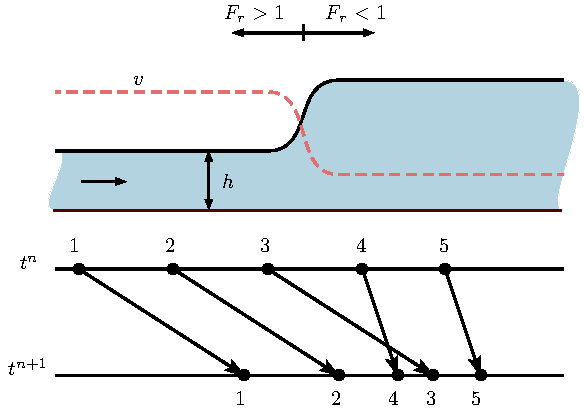
\includegraphics[width=.8\textwidth]{img/lagrangian/pfem_shock.pdf}
    \caption{Incompatibility of the mesh moving algorithm for solving problems with shocks.}
    \label{pfem_shock}
\end{figure}

While the primitive variables are not optimal to solve shocks, the mesh moving algorithm presents another difficulty.
Both methods present restrictions, but the nature of that difficulties are different. The restriction of the primitive variables is related to the conservation of the momentum at discrete level. The restriction of the mesh moving algorithm is associated to the finite differencing convective operator.





\section{Fixed mesh methods}


In this section a Lagrangian procedure with fixed mesh is presented. This procedure is an extension of PFEM-2 \cite{idelsohn2012} to the SW equations. In contrast to the mesh moving algorithm, the particles does not coincide with the nodes, but they move over the FE mesh. This procedure has the advantage of avoiding the remeshing step, but the cost of a projection from the particles to the mesh.

Let $\mathcal{P}$ be a set of particles randomly seed over the SW domain. The density of the particles is such that the average number of particles per element is greater than one. This particles move over the domain transporting the intrinsic variables of the fluid, namely density, water depth, flow rate, etc. This convection stage is finalized with a projection of the variables of the particles to the FE mesh.
The solution of the step is completed with the FE counterpart, solved in the fixed mesh following a Lagrangian framework. Finally, updating the particles is a trivial operation since the FE interpolation allows to evaluate the unknowns at an arbitrary point, namely, the particles.
Figure \ref{pfem2_stage_flowchart} summarizes the main stages of the PFEM-2 algorithm.


\begin{figure}
    \centering
    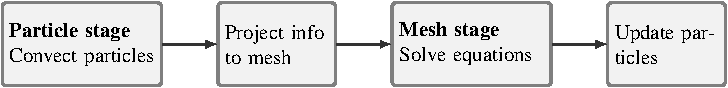
\includegraphics[width=\textwidth]{img/lagrangian/pfem2_stage_flowchart.pdf}
    \caption{PFEM-2 flowchart}
    \label{pfem2_stage_flowchart}
\end{figure}


In the same way as the mesh moving algorithm, this scheme may undergo certain variations. Strictly speaking, the mass and momentum balance are a coupled system of equations and the Lagrangian split does not modify that property. This will be analyzed in the following sections.



\subsection{Governing equations}


In contrast to the moving mesh algorithm, the nodes receive information from the particles without experimenting mesh displacement.
This fact allows to arbitrarily choose a Lagrangian or Eulerian framework, even for only one of the balance equations.
This property of the PFEM-2 algorithm allows more flexibility. The choose of the equations as well as the framework can optimize the computational cost and the approximation of the physical properties.
For example, Heniche pointed out in \cite{heniche2000} that the residual of the momentum balance does not distinguish the sign of the water depth if conservative variables are employed, $\mathbf{r}_\mathbf{q}(h) = \mathbf{r}_\mathbf{q}(-h)$.
This property suggests the use of conservative variables in combination with a mixed framework.
\begin{subequations} \label{pfem2_sw_eq}
\begin{align}
    &\frac{D\mathbf{q}}{Dt} + \mathbf{q} \nabla \cdot \mathbf{u} + gh \nabla (h-z) + S_f = \mathbf{0} \\
    &\pder{h}{t} + \nabla \cdot \mathbf{q} = 0
\end{align}
\end{subequations}


The first term involving spatial derivatives in the momentum balance comes from applying the chain rule to the fluxes vector and subtracting the convective term. The remaining terms corresponds to the compressibility of the SW equations --it is important to remember the analogy between the SW equations and the compressible NS equations--.

Several possibilities are presented to deal with this term. The first one consists on recovering the Eulerian quasi-linear form and then, apply the material derivative. The second one imply a projection to compute the divergence of the velocity. Lastly, an updated Lagrangian formulation can be used to compute the divergence term.

The first option is preferred since it is more consistent with the previous sections and does not introduce extra steps. The linearization matrices follow the next expression:
\begin{equation}
    \mathbf{A}_1 = \left[\begin{matrix}
        u_1  & 0   & -u_1^2 + gh \\
        u_2  & 0   & -u_1 u_2 \\
        1    & 0   & 0
    \end{matrix} \right]
    \quad , \quad
    \mathbf{A}_2 = \left[\begin{matrix}
        0   & u_1  & -u_1 u_2 \\
        0   & u_2  & -u_2^2 + gh \\
        0   & 1    & 0
    \end{matrix} \right]
\end{equation}




\subsection{PFEM-2 algorithm}


The outlined algorithm is explained in more detail in the section. The more important parts are the computations carried out by each discrete space. The communication between them and the integration in time are strictly related.


\subsubsection{Convection}


Let us assume that the particles move as material points and that each one stores the point concentration of the property $\phi_p = \phi(\mathbf x_p)$. Since the variables are not known for any arbitrary time $t$, but only for the discrete time steps $1,\ 2\dots n,\ n+1\dots$, the advection of a particle can be approximated using a $\theta$-family discretization as:
\begin{equation}
\mathbf{x}_p^{n+1} = \mathbf{x}_n^p + (1-\theta) \int_{t_n}^{t_{n+1}} \mathbf{v}_n(\mathbf{x}_p^t)dt + \theta \int_{t_n}^{t_{n+1}} \mathbf{v}_{n+1}(\mathbf{x}_p^t)dt
\end{equation}

If the velocity field is known, the system becomes explicit and the problem is reduced to moving the particles along the streamlines. The problem is solved using an explicit forward integration ($\theta=0$) with a proper sub-step \cite{idelsohn2012}. An illustration is given in figure \ref{pfem2_convection_stage}. This method, also known as XIVAS \cite{idelsohn2013}\cite{idelsohn2014}, was initially applied to a variable velocity field.
After the particles are moved, the ones that leave the domain are removed.

In this work the computational domain is initially seeded with fifteen particles per element. This number does not remain constant during the simulation because particles can freely enter and exit finite elements as they move through the domain. Thereby, in order to properly perform the advection stage, every time step the domain is reseed with particles so as to ensure that a minimum number is present within each finite element. This number of particles was chosen to be four. Particles can also be eliminated from each finite element in order to limit the computational cost. In this case, the maximum number of particles allowed per finite element is sixteen. These particle thresholds were chosen as they have proven to give accurate results in previous works \cite{idelsohn2015}.

\begin{figure} [htb]
\begin{subfigure}{0.48\textwidth}
    \centering
    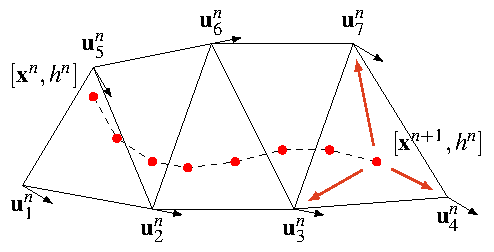
\includegraphics[width=\textwidth]{img/lagrangian/pfem2_convection_stage.pdf}
    \caption{Explicit advection stage using particles (in red). Next, the particles' information is transferred to the mesh nodes.}
    \label{pfem2_convection_stage}
\end{subfigure}
\hfill
\begin{subfigure}{0.48\textwidth}
    \centering
    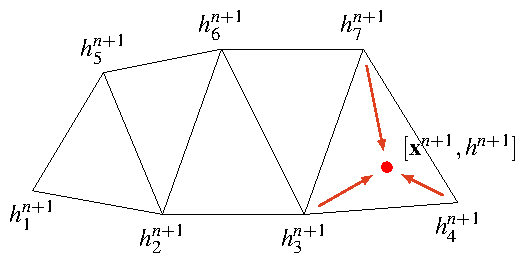
\includegraphics[width=\textwidth]{img/lagrangian/pfem2_wave_stage.pdf}
    \caption{After the computation of the wave stage, the FE nodes contribute to the particles.}
    \label{pfem2_wave_stage}
\end{subfigure}
\caption{Illustration of the two main steps of the PFEM2 framework.}
\label{pfem2_diffusion_and_wave_stages}
\end{figure}



\subsubsection{Projection}


When solving the advective stage in Equation (\ref{pfem2_sw_eq}), the particles concentration at $\mathbf x_p^{n+1}$ is the same as at the onset of the time step ($\mathbf x_p^n$). This is equivalent to saying that the advective step assumes $\frac{D\phi}{D t}=0$. This modification in the field described by the particles needs to be transferred onto the finite element space. As usual in particle-based techniques, such as PFEM, a projection procedure is used to transfer the information from the particles to the finite elements in the underlying mesh. In our work we use

\begin{equation}
    \phi^* = \mathcal L(\phi_p)
\end{equation}

where $\mathcal L$ is the projection operator from the particles to the finite element space and $\phi^*$ is the result of the advection at the time step $n+1$. In this case, a first order explicit projection has been used and all the particles in the elements surrounding a node contribute to that node, i.e.
%TODO: ($\theta = ? $)

\begin{equation}
    \phi_i^* = \dfrac
    {\Sigma_e\Sigma_{p_e} w_p \phi_p}
    {\Sigma_e\Sigma_{p_e} w_p}
    \quad \text{with} \quad
    w_p = N_{ei}(\mathbf x_p)
\end{equation}

where the index $i$ runs over all the mesh nodes, where $e$ runs over the elements sharing node $i$ and where $p_e$ runs over the particles contained in element $e$.


\begin{figure} [htb]
\begin{subfigure}{0.47\textwidth}
    \centering
    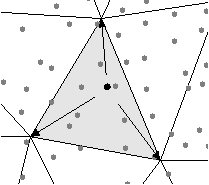
\includegraphics[width=\textwidth]{img/lagrangian/projection.pdf}
    \caption{Each particle contribute to the nodes from its element.}
    \label{pfem2_projection}
\end{subfigure}
\hfill
\begin{subfigure}{0.47\textwidth}
    \centering
    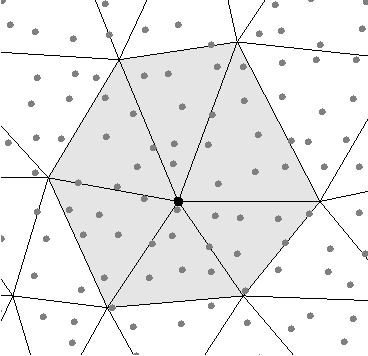
\includegraphics[width=\textwidth]{img/lagrangian/projection_full.pdf}
    \caption{Kernel of elements and particles contributing to a node.}
    \label{pfem2_projection_full}
\end{subfigure}
\caption{Illustration of the projection stage of the PFEM2 framework.}
\label{pfem2_projection_full_illustrations}
\end{figure}


\subsubsection{Wave equation stage}


Once the convective problem is solved explicitly in the particles and the results are transferred to the mesh nodes, the lagrangian residual (Equation (\ref{pfem2_sw_eq})) is solved in a fixed mesh with an Eulerian FIC-FEM technique. The spatial discretization and the time integration scheme follows the procedure explained in Section \ref{sec:fic_fem_stabilization}.
However, the time integration scheme follows a first-order BDF or Backward Euler.
The time derivatives are computed according to the next expressions
\begin{align} \label{pfem2_time_derivatives}
    \dot{\mathbf{q}} &= \frac{\mathbf{q}^{n+1} - \mathbf{q}^*}{\Delta t} \\
    \dot{h} &= \frac{h^{n+1} - h^n}{\Delta t}
\end{align}
Equation (\ref{pfem2_time_derivatives}) includes the contribution of the advection computed with the particles through the variables $^*$. It is important to note that the water depth is still using a partial derivative.

Another minor modification with respect to the Eulerian framework, is the use of the convected values as initial guess for the iterative strategy:
\begin{align}
    \mathbf{q}^{n+1,0} = \mathbf{q}^* \\
    h^{n+1,0} = h^*
\end{align}

Finally, it is worth to remark the need of stabilization, since the discretization does not fulfill the compatibility of interpolation. Though, several authors report instabilities but does not associate them to the \emph{inf-sup} condition. The stability is introduced following the procedure explained in section \ref{sec:fic_fem_stabilization}.


\subsubsection{Particles update}
The last step of the PFEM2 algorithm is to add the contribution of the solution of Equation (\ref{pfem2_sw_eq}) to the particles. To avoid the accumulation of projection errors and additional diffusion, the information from the particles is updated using an incremental scheme. This step only involves the evaluation of the unknown at each particle position in the finite element mesh as:

\begin{equation}
    \phi_p^{n+1} = \phi_p^n + \phi({\bf x}_p^{n+1}) - \phi({\bf x}_p^*)
\end{equation}



\section{Examples}


In this section an example is presented as a proof of concept of the Lagrangian methods. Its advantages and drawbacks compared to the Eulerian framework are discussed. Here, the example presented in section \ref{sec:examples:parabola} is taken up again, since the oscillation benchmark is a good option to test the accuracy of the shoreline tracking.

As a reminder, this benchmark has been extracted from \cite{delestre2013} and has an analytical solution. The problem consists on a 1D parabolic basin containing a mass of water. The initial condition is zero velocity and the free surface describing an inclined plane. After the initial time $t=0$, the mass of water begins to slice over the parabolic basin and describes an oscillatory movement. The topography is described in equation (\ref{eq:parabola:topography}) and the analytical solution follows equation (\ref{eq:parabola:variables}). The same parameters than the ones in section \ref{sec:examples:parabola} are used in this example:
\begin{equation*}
    h_0 = 1 \quad,\quad a = 1
\end{equation*}

The spatial domain is $\Omega=[0,10]\times[0,1]m^2$, where the parabola is aligned with the larges dimension. 
Figure \ref{fig:pfem_parabola_view} shows the discretization of the problem using the PFEM algorithm. For visualization purpose, the meshes are deformed vertically with the topography and the free surface respectively.

\begin{figure}
    \centering
    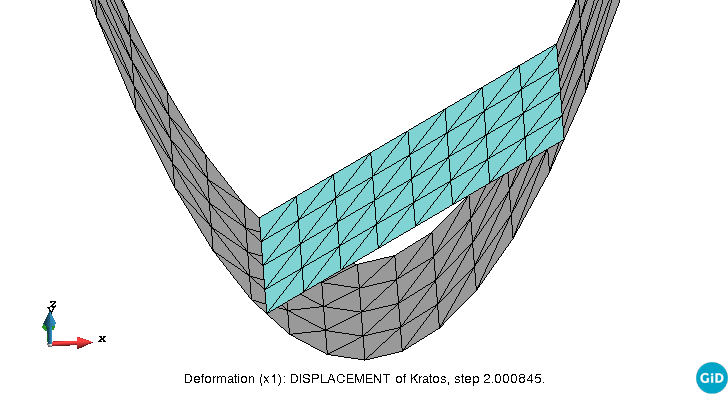
\includegraphics[width=.8\textwidth]{img/lagrangian/parabola_view.png}
    \caption{Detail of the discretizations used to solve the oscillation in a parabolic basin with the mesh moving algorithm (PFEM).}
    \label{fig:pfem_parabola_view}
\end{figure}



\begin{figure}
    \centering
    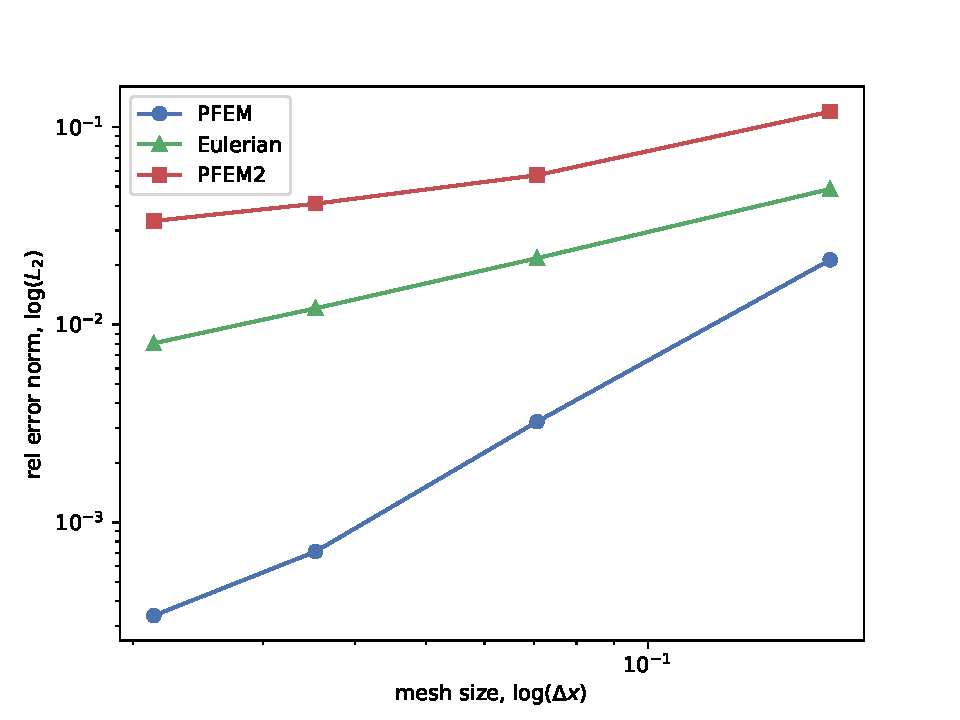
\includegraphics[width=.7\textwidth]{img/lagrangian/convergence}
    \caption{Comparison of the convergence for the presented methods.}
    \label{fig:lagrangian_parabola_convergence}
\end{figure}


A convergence analysis has been carried out with the proposed method and the results are summarized in Figure \ref{fig:lagrangian_parabola_convergence}. As expected, the order of convergence of the PFEM method is not affected by the moving shoreline, keeping the second order of the FE formulation.





\section{Concluding remarks}


Lagrangian methods exhibit some computational benefits but the main advantage is its natural tracking of the shoreline. Especially the mesh moving algorithm, does not need additional treatment since it is not affected by the dry domain. The main drawback of the Lagrangian methods is related to the compressible behavior of the SW equations. On the on side, the velocity field is discontinuous around shocks and the staggered character of the time strategy is not suited to this phenomena. Furthermore, the explicit calculation of the convection faces a strong restriction on the CFL number.
On the other side, the Lagrangian formulation does not achieve the desired linearization when compressible formulations are considered.
Figure \ref{pfem_euler_convergence} shows a schematic of the order of convergence in terms of the Froude number. When the Froude number is equal to 1, there is a discontinuity. The moving shoreline is characterized by a very elevated Froude number, since the shoreline involves a quasi zero water depth.

\begin{figure}
    \centering
    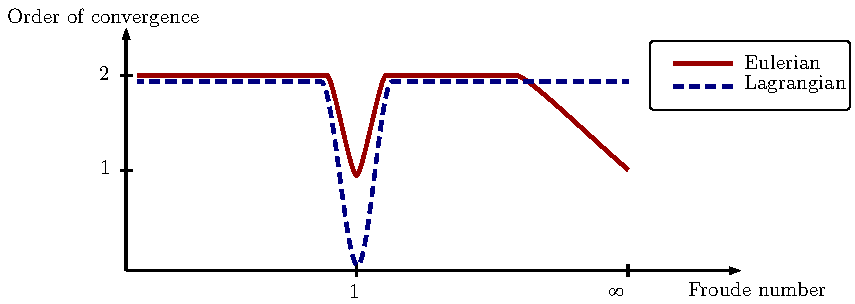
\includegraphics[width=\textwidth]{img/lagrangian/lagrangian_eulerian_convergence.pdf}
    \caption{Qualitative representation of the order of convergence in terms of the Froude number.}
    \label{pfem_euler_convergence}
\end{figure}


A global overview of the Lagrangian and Eulerian methods identifies the Eulerian framework as the robust one. Nevertheless, the Lagrangian framework is still interesting for the shoreline tracking.
A promising combination would be an arbitrary Lagrangian-Eulerian formulation using the Eulerian framework where shocks and oscillatory behavior is dominant, and using a Lagrangian framework where the shoreline is moving.

